\chapter{Appendix B. BASESIMP foundation configurations} \label{Appendix:BasesimpConfigurations}

BASESIMP is developed to model a large variety of foundation types and insulation configuration representing the majority of the Canadian housing stock.  The possible configurations are reproduced in this Appendix. All configurations are assigned a code including three (for slab-in-grade foundations) or four (for basements) letters and a number where:
\begin{flushleft}
\begin{itemize}
    \item[-] The first letter represents the foundation type: B = Basement; S = Slab-in-grade;
    \item[-] The second letter represents the foundation construction: C = Concrete; W = Wood; B = Wood walls and Concrete slab;
    \item[-] The third (for basements) letter represents the wall insulation: N = None; I = Interior; E = Exterior; C = Interior and Exterior;
    \item[-] The third (for slabs) or fourth (for basements) letter represents the floor insulation: N = None; A = Above; B = Below;
    \item[-] The number is an identifier.
\end{itemize}
\end{flushleft}

\noindent All possible basement configurations have common characteristics:
\begin{flushleft}
\begin{itemize}
    \item[-] Concrete basements have $200 \: mm$ walls and $100 \: mm$ floors;
    \item[-] Wood basements have $50 \: mm$ walls and $100 \: mm$ floors;
    \item[-] Configurations can account for a first-storey brick veneer placed directly on basement’s concrete walls (see Figure \ref{fig:UninsulatedBasements});
    \item[-] Wall interior insulation can cover: the entire height of the wall; from the top to $0.2 \: m$ above the floor; from top of wall to $0.6 \: m$ below-grade;
    \item[-] Wall exterior insulation can cover: the entire height of the wall; the below grade part of the wall; from top of wall to $0.6 \: m$ below-grade;
    \item[-] When the walls and the floor are insulated, they have the same thermal resistance;
    \item[-] Above floor insulation can cover: the entire floor; or a $0.6 \: m$ strip around the perimeter;
    \item[-] Below floor insulation can cover: the entire floor; a $0.6 \: m$ strip around the perimeter; or a $1.0 \: m$ strip around the perimeter;
\end{itemize}
\end{flushleft}

%Configurations BCCN-1, BCCN-2, and BCCA-1 have the particularity that the %user can determine the width of the overlap between the interior and %exterior wall insulations.  The exterior insulation covers the below grade %portion of the wall.  Adjusting this overlap provides the user with a %measure of control over the height of the interior insulation.

\section{Basements}

\begin{figure} [htb]
      \subfigure[BCNN-1 (brick veneer)]{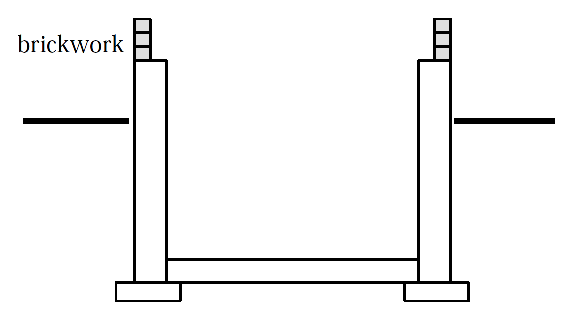
\includegraphics[width=0.45\textwidth]{BSCONFIG-BCNN_1.png}}\hfil
      \subfigure[BCNN-2 (no brick veneer)]{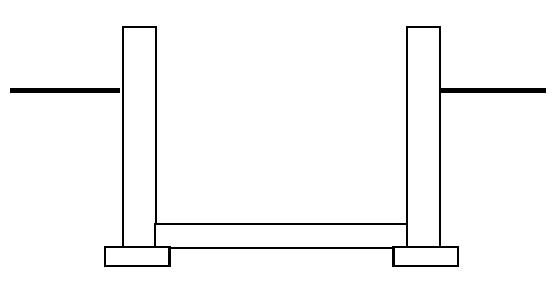
\includegraphics[width=0.45\textwidth]{BSCONFIG-BCNN_2.png}}
      \caption{Concrete basements with no insulation} \label{fig:UninsulatedBasements}
\end{figure}

\begin{figure} [htb]
      \subfigure[BCIN-1]{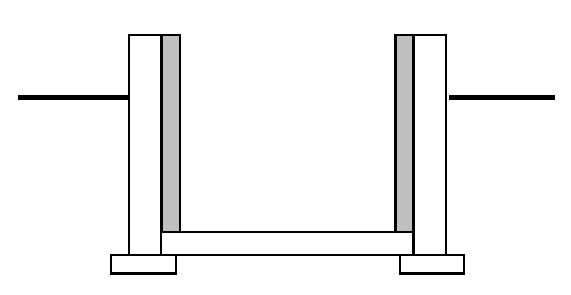
\includegraphics[width=0.45\textwidth]{BSCONFIG-BCIN_1.png}}\hfil
      \subfigure[BCIN-2]{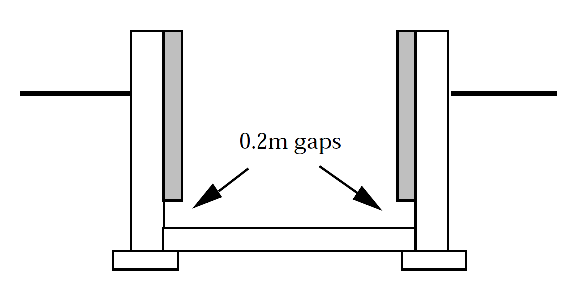
\includegraphics[width=0.45\textwidth]{BSCONFIG-BCIN_2.png}}
    \\
      \subfigure[BCIN-3]{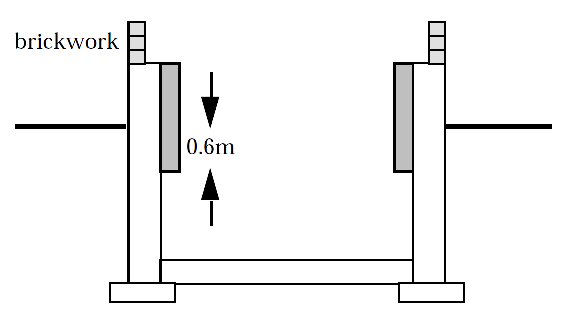
\includegraphics[width=0.45\textwidth]{BSCONFIG-BCIN_3.png}}\hfil
      \subfigure[BCIN-4]{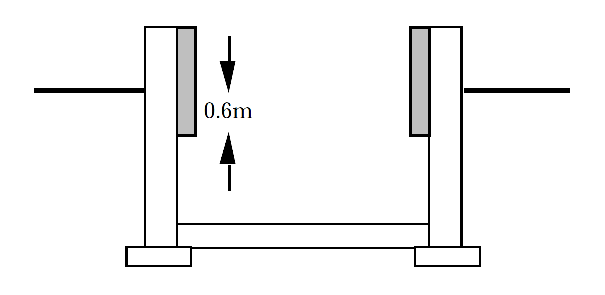
\includegraphics[width=0.45\textwidth]{BSCONFIG-BCIN_4.png}}
    \caption{Concrete basements with interior wall insulation}
\end{figure}

\newpage

\begin{figure} [htb]
      \subfigure[BCEN-1]{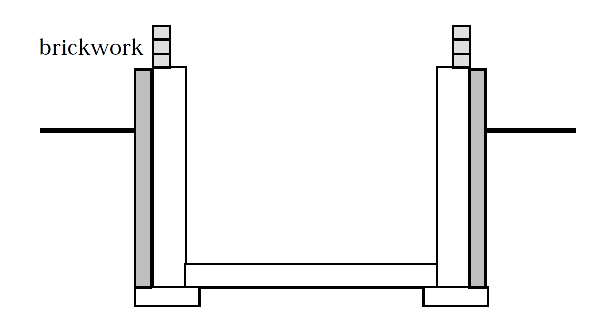
\includegraphics[width=0.48\textwidth]{BSCONFIG-BCEN_1.png}}\hfil
      \subfigure[BCEN-2]{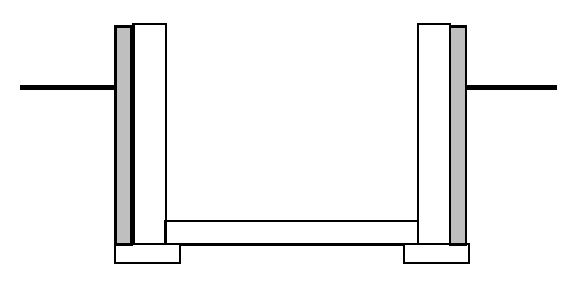
\includegraphics[width=0.48\textwidth]{BSCONFIG-BCEN_2.png}}
    \\
      \subfigure[BCEN-3]{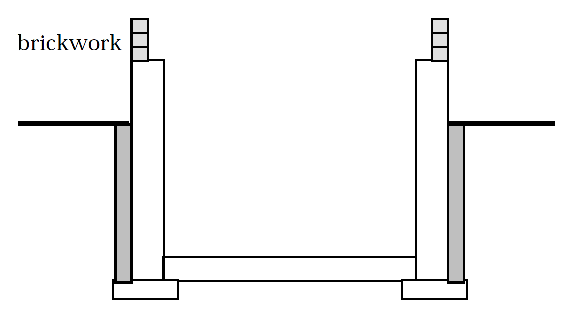
\includegraphics[width=0.48\textwidth]{BSCONFIG-BCEN_3.png}}\hfil
      \subfigure[BCEN-4]{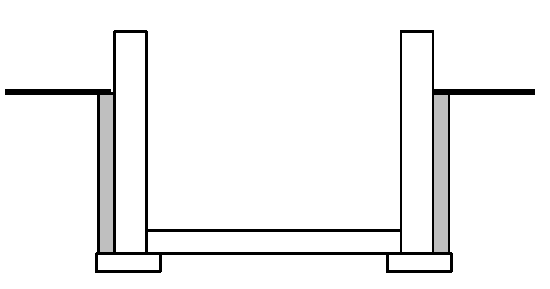
\includegraphics[width=0.48\textwidth]{BSCONFIG-BCEN_4.png}}
    \\
      \subfigure[BCEN-5]{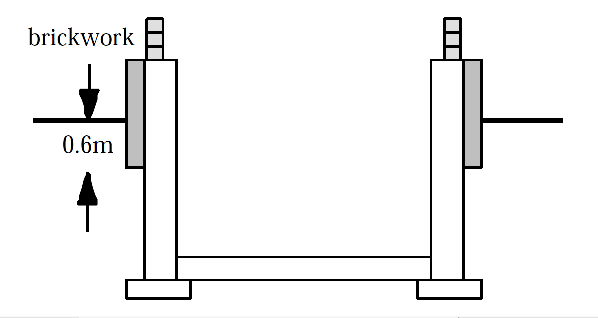
\includegraphics[width=0.48\textwidth]{BSCONFIG-BCEN_5.png}}\hfil
      \subfigure[BCEN-6]{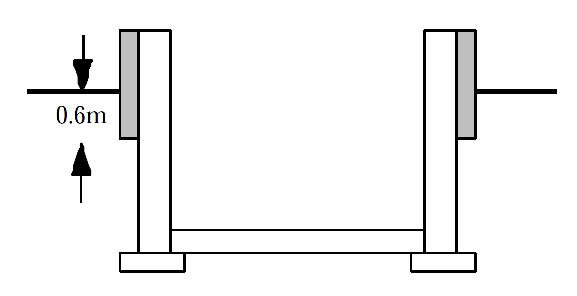
\includegraphics[width=0.48\textwidth]{BSCONFIG-BCEN_6.png}}
    \caption{Concrete basements with exterior wall insulation}
\end{figure}

\newpage

\begin{figure} [htb]
      \subfigure[BCCN-1]{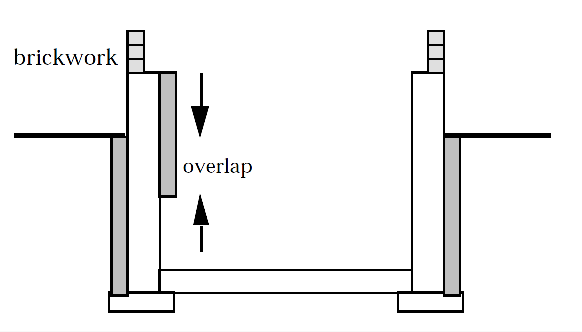
\includegraphics[width=0.48\textwidth]{BSCONFIG-BCCN_1.png}}\hfil
      \subfigure[BCCN-2]{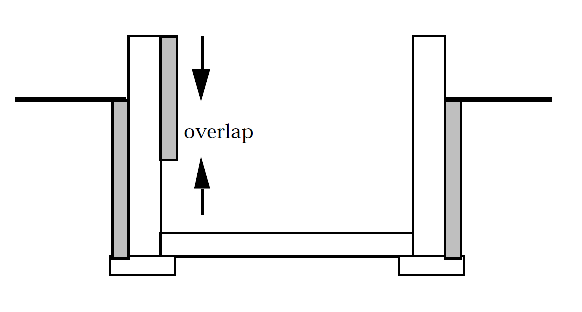
\includegraphics[width=0.48\textwidth]{BSCONFIG-BCCN_2.png}}
    \\
      \subfigure[BCCN-3]{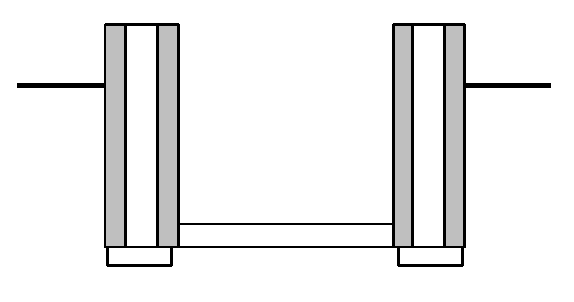
\includegraphics[width=0.48\textwidth]{BSCONFIG-BCCN_3.png}}\hfil
      \subfigure[BCCN-4]{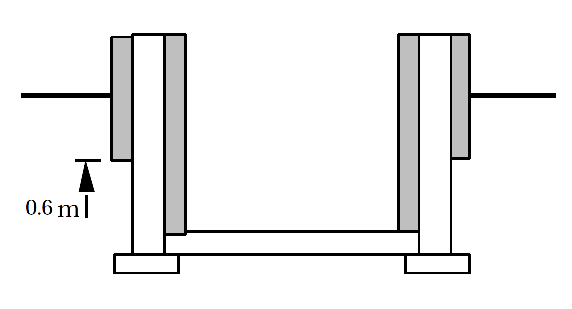
\includegraphics[width=0.48\textwidth]{BSCONFIG-BCCN_4.png}}
    \\
      \subfigure[BCCN-5]{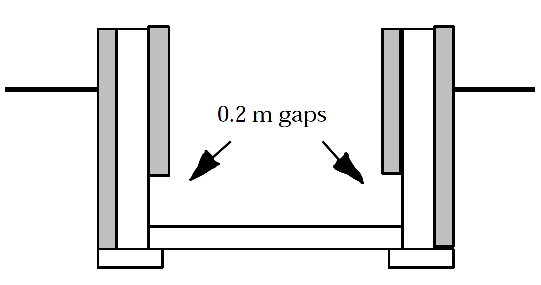
\includegraphics[width=0.48\textwidth]{BSCONFIG-BCCN_5.png}} \hfil
      \caption{Concrete basements with interior and exterior wall insulation}
\end{figure}

\newpage

\begin{figure} [htb]
      \subfigure[BCIB-1]{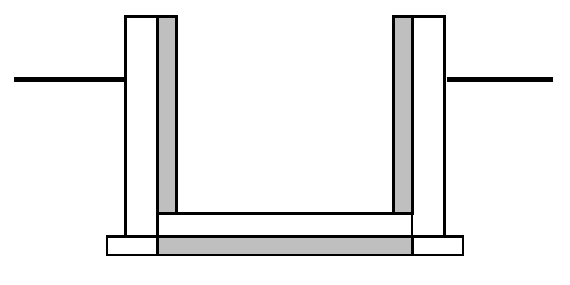
\includegraphics[width=0.33\textwidth]{BSCONFIG-BCIB_1.png}}\hfil
      \subfigure[BCIB-2]{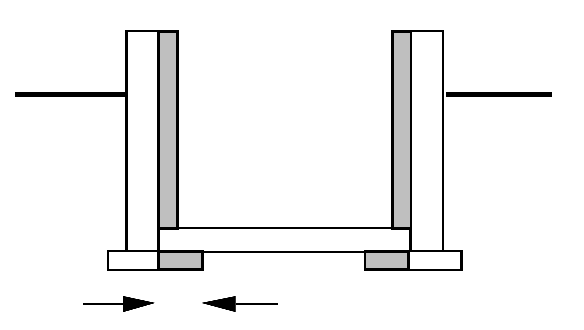
\includegraphics[width=0.33\textwidth]{BSCONFIG-BCIB_2.png}}
    \\
      \subfigure[BCIB-3]{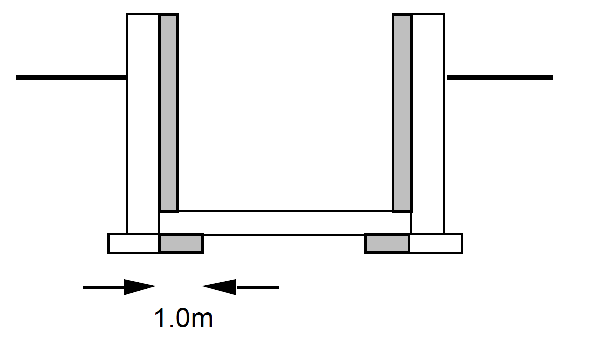
\includegraphics[width=0.33\textwidth]{BSCONFIG-BCIB_3.png}}\hfil
      \subfigure[BCIB-4]{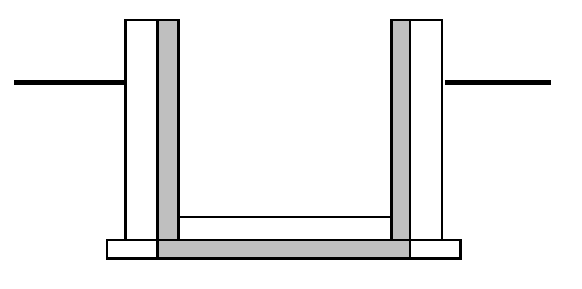
\includegraphics[width=0.33\textwidth]{BSCONFIG-BCIB_4.png}}
    \\
      \subfigure[BCIB-5]{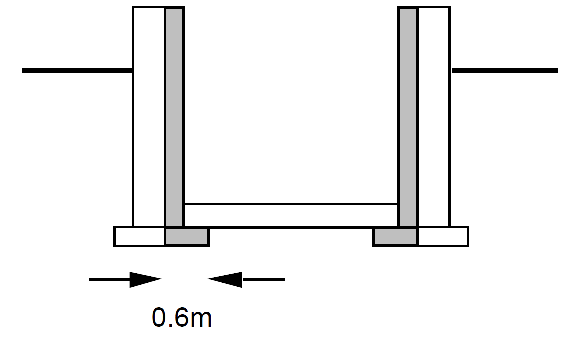
\includegraphics[width=0.33\textwidth]{BSCONFIG-BCIB_5.png}}\hfil
      \subfigure[BCIB-6]{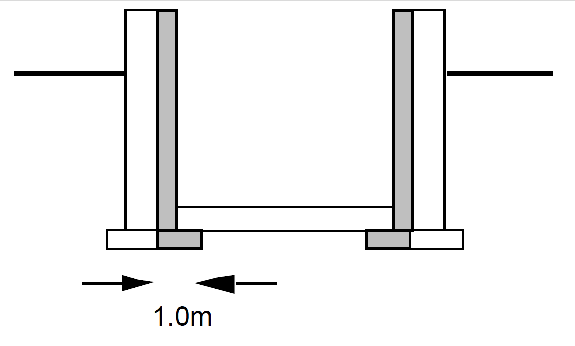
\includegraphics[width=0.33\textwidth]{BSCONFIG-BCIB_6.png}}
    \\
      \subfigure[BCIB-7]{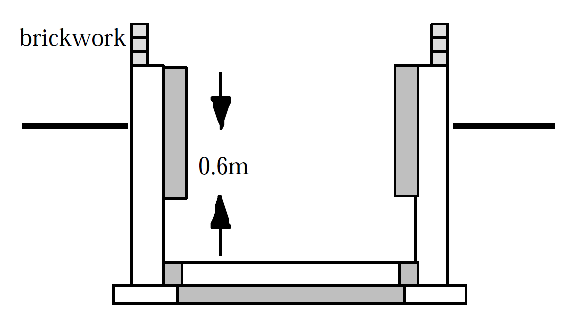
\includegraphics[width=0.33\textwidth]{BSCONFIG-BCIB_7.png}}\hfil
      \subfigure[BCIB-8]{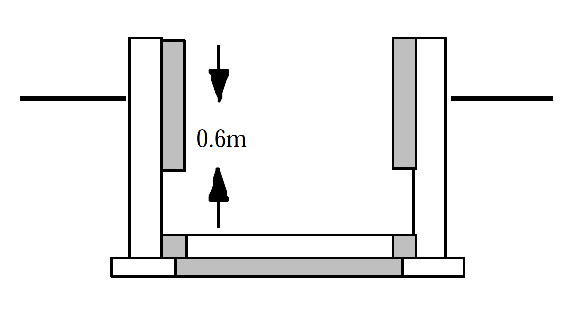
\includegraphics[width=0.33\textwidth]{BSCONFIG-BCIB_8.png}}
    \caption{Concrete basements with interior wall and under-floor insulation}
\end{figure}

\newpage

\begin{figure} [htb]
      \subfigure[BCEB-1]{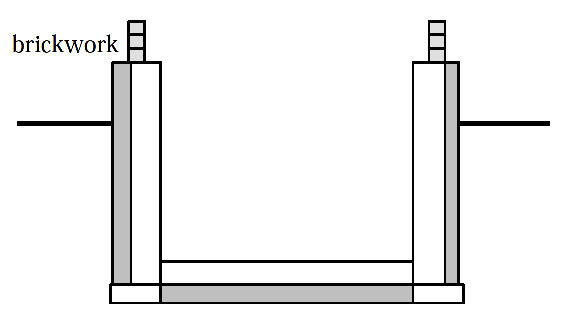
\includegraphics[width=0.30\textwidth]{BSCONFIG-BCEB_1.png}}\hfil
      \subfigure[BCEB-2]{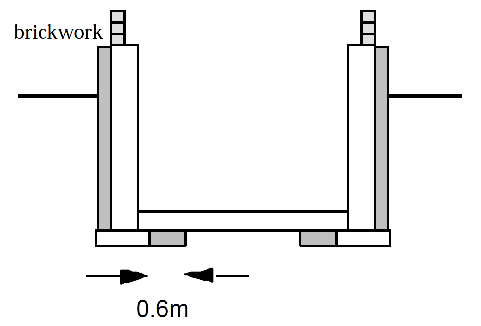
\includegraphics[width=0.30\textwidth]{BSCONFIG-BCEB_2.png}}
    \\
      \subfigure[BCEB-3]{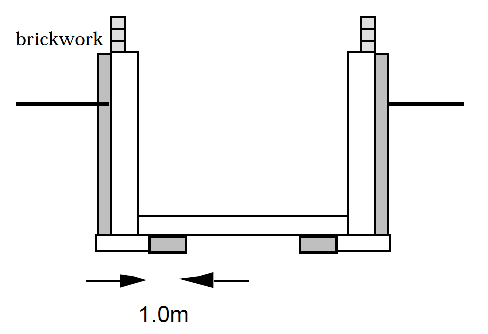
\includegraphics[width=0.30\textwidth]{BSCONFIG-BCEB_3.png}}\hfil
      \subfigure[BCEB-4]{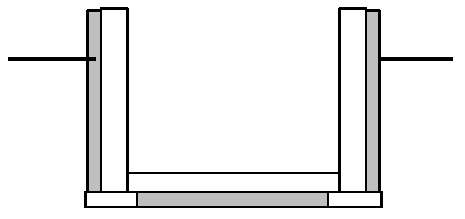
\includegraphics[width=0.30\textwidth]{BSCONFIG-BCEB_4.png}}
    \\
      \subfigure[BCEB-5]{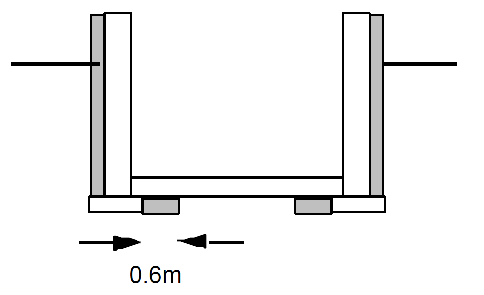
\includegraphics[width=0.30\textwidth]{BSCONFIG-BCEB_5.png}}\hfil
      \subfigure[BCEB-6]{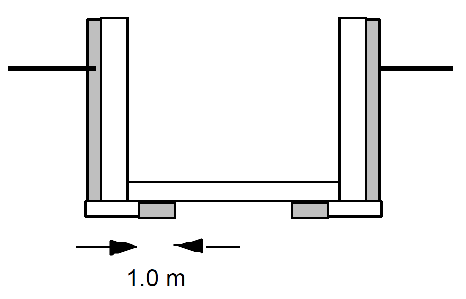
\includegraphics[width=0.30\textwidth]{BSCONFIG-BCEB_6.png}}
    \\
      \subfigure[BCEB-8]{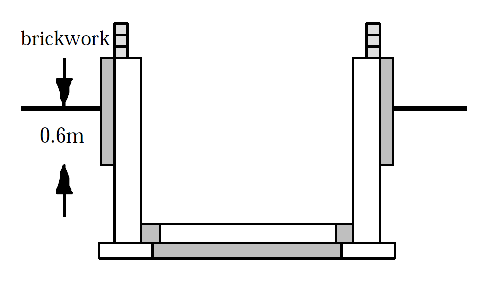
\includegraphics[width=0.30\textwidth]{BSCONFIG-BCEB_8.png}}\hfil
      \subfigure[BCEB-9]{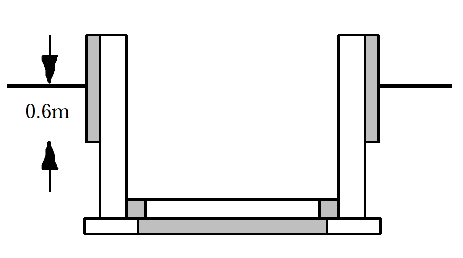
\includegraphics[width=0.30\textwidth]{BSCONFIG-BCEB_9.png}}
     \caption{Concrete basements with exterior wall and under-floor insulation}
\end{figure}

\newpage

\begin{figure} [htb]
      \subfigure[BCCB-4]{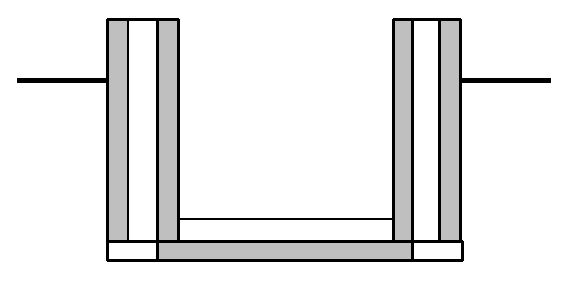
\includegraphics[width=0.43\textwidth]{BSCONFIG-BCCB_4.png}}\hfil
      \subfigure[BCCB-8]{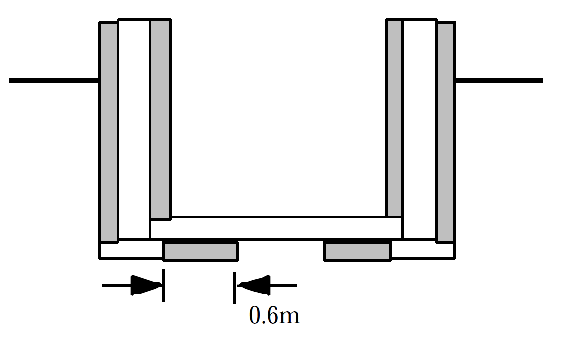
\includegraphics[width=0.43\textwidth]{BSCONFIG-BCCB_8.png}}
    \\
      \subfigure[BCCB-9]{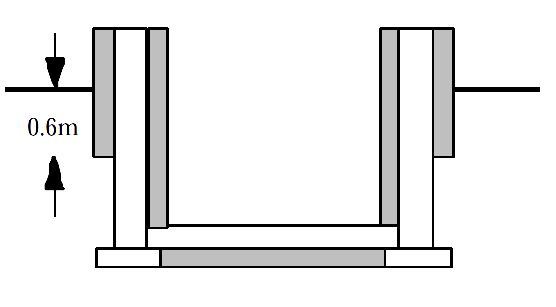
\includegraphics[width=0.43\textwidth]{BSCONFIG-BCCB_9.png}}\hfil
      \subfigure[BCCB-10]{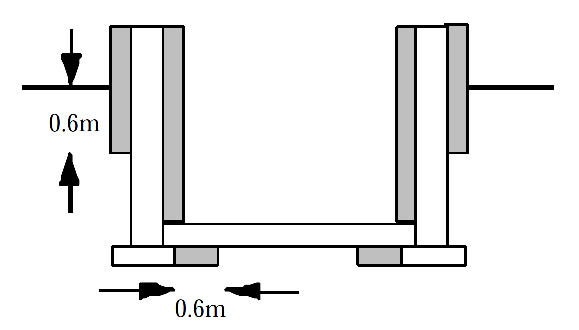
\includegraphics[width=0.43\textwidth]{BSCONFIG-BCCB_10.png}}
    \caption{Concrete basements with interior and exterior wall insulation and under-floor insulation}
\end{figure}

\begin{figure} [htb]
      \subfigure[BCIA-1]{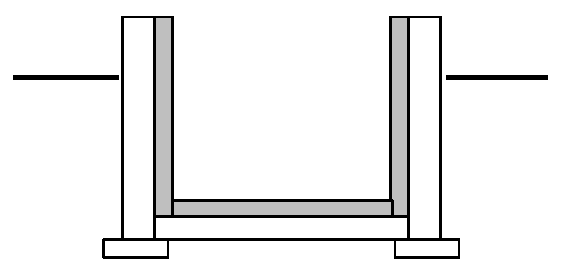
\includegraphics[width=0.43\textwidth]{BSCONFIG-BCIA_1.png}}\hfil
      \subfigure[BCIA-4]{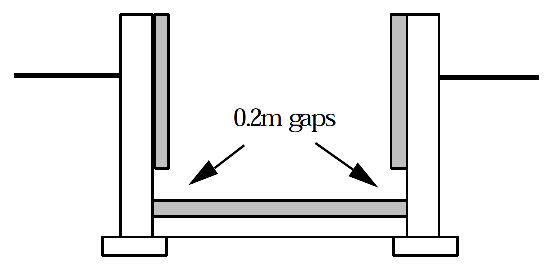
\includegraphics[width=0.43\textwidth]{BSCONFIG-BCIA_4.png}}
      \caption{Concrete basements with interior wall and above-floor insulation}
\end{figure}

\newpage

\begin{figure} [htb]
      \subfigure[BCEA-1]{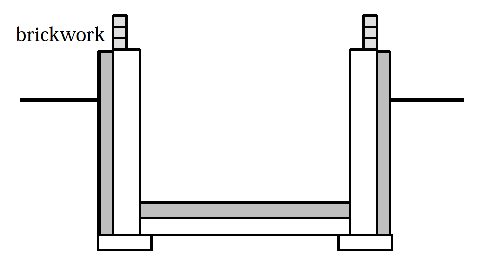
\includegraphics[width=0.48\textwidth]{BSCONFIG-BCEA_1.png}}\hfil
      \subfigure[BCEA-4]{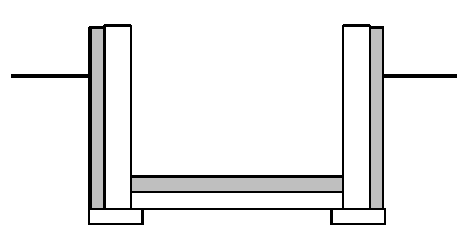
\includegraphics[width=0.48\textwidth]{BSCONFIG-BCEA_4.png}}
    \\
      \subfigure[BCEA-5]{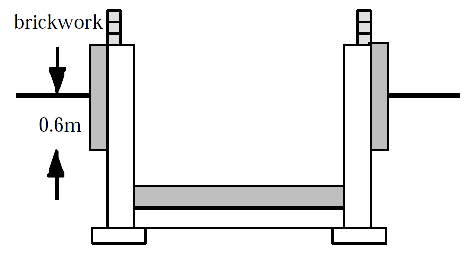
\includegraphics[width=0.48\textwidth]{BSCONFIG-BCEA_5.png}}\hfil
      \subfigure[BCEA-6]{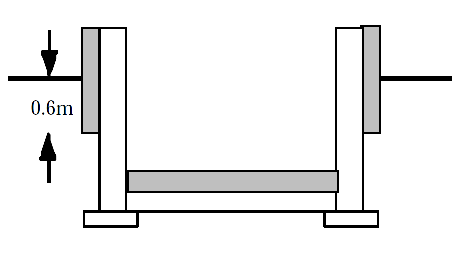
\includegraphics[width=0.48\textwidth]{BSCONFIG-BCEA_6.png}}
    \\
      \subfigure[BCEA-7]{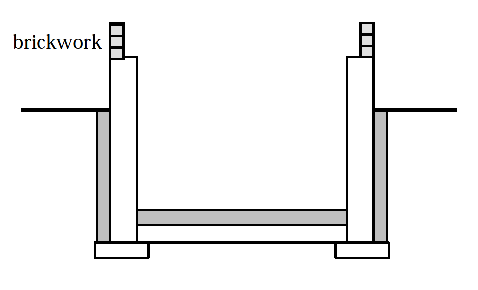
\includegraphics[width=0.48\textwidth]{BSCONFIG-BCEA_7.png}}\hfil
      \subfigure[BCEA-8]{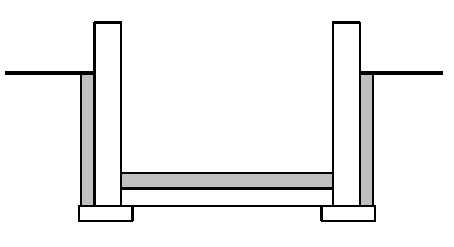
\includegraphics[width=0.48\textwidth]{BSCONFIG-BCEA_8.png}}
     \caption{Concrete basements with exterior wall and above-floor insulation}
\end{figure}

\newpage

\begin{figure} [htb]
      \subfigure[BCCA-1]{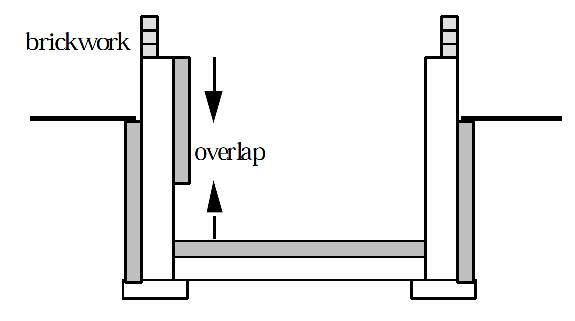
\includegraphics[width=0.48\textwidth]{BSCONFIG-BCCA_1.png}}\hfil
      \subfigure[BCCA-4]{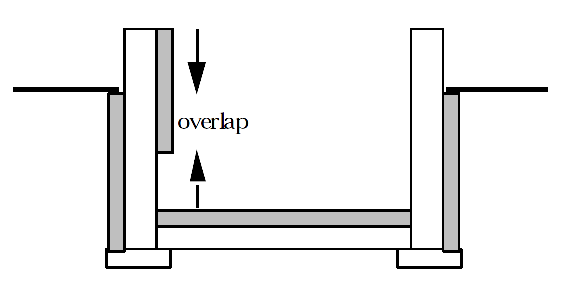
\includegraphics[width=0.48\textwidth]{BSCONFIG-BCCA_4.png}}
    \\
      \subfigure[BCCA-7]{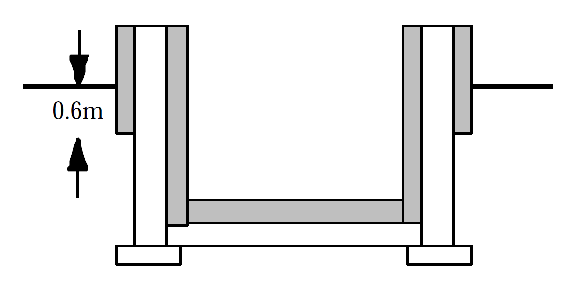
\includegraphics[width=0.48\textwidth]{BSCONFIG-BCCA_7.png}}\hfil
      \subfigure[BCCA-8]{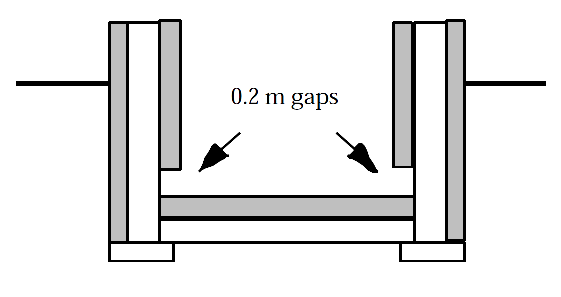
\includegraphics[width=0.48\textwidth]{BSCONFIG-BCCA_8.png}}
    \caption{Concrete basements with interior and exterior wall and above-floor insulation} \label{fig:concBasementIntExtAboveIns}
\end{figure}

\newpage

\begin{figure} [htb]
      \subfigure[BWNN-1]{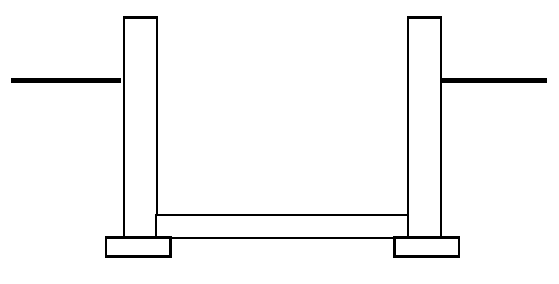
\includegraphics[width=0.48\textwidth]{BSCONFIG-BWNN_1.png}}\hfil
      \subfigure[BWIN-1]{\includegraphics[width=0.48\textwidth]{BSCONFIG-BWIN_1.png}}
    \\
      \subfigure[BWIN-2]{\includegraphics[width=0.48\textwidth]{BSCONFIG-BWIN_2.png}}\hfil
      \subfigure[BWIN-3]{\includegraphics[width=0.48\textwidth]{BSCONFIG-BWIN_3.png}}
    \\
      \subfigure[BWIA-1]{\includegraphics[width=0.48\textwidth]{BSCONFIG-BWIA_1.png}}\hfil
      \subfigure[BWIA-2]{\includegraphics[width=0.48\textwidth]{BSCONFIG-BWIA_2.png}}
    \caption{Wood basements}\label{fig:woodBasementsConfig}
\end{figure}

\newpage

\begin{figure} [htb]
      \subfigure[BBIN-1]{\includegraphics[width=0.39\textwidth]{BSCONFIG-BBIN_1.png}}\hfil
      \subfigure[BBIN-2]{\includegraphics[width=0.39\textwidth]{BSCONFIG-BBIN_2.png}}
     \caption{Combination basements with interior wall insulation}
\end{figure}

\begin{figure} [htb]
      \subfigure[BBEN-1]{\includegraphics[width=0.39\textwidth]{BSCONFIG-BBEN_1.png}}\hfil
      \subfigure[BBEN-2]{\includegraphics[width=0.39\textwidth]{BSCONFIG-BBEN_2.png}}
     \caption{Combination basements with exterior wall insulation} \label{fig:mixedBasementsConfigBegin}
\end{figure}

\begin{figure} [htb]
      \subfigure[BBIA-1]{\includegraphics[width=0.39\textwidth]{BSCONFIG-BBEB_1.png}}\hfil
      \subfigure[BBIA-2]{\includegraphics[width=0.39\textwidth]{BSCONFIG-BBEB_2.png}}
     \caption{Combination basements with interior wall and above-floor insulation}
\end{figure}

\newpage

\begin{figure} [htb]
      \subfigure[BBIB-1]{\includegraphics[width=0.43\textwidth]{BSCONFIG-BBIB_1.png}}\hfil
      \subfigure[BBIB-2]{\includegraphics[width=0.43\textwidth]{BSCONFIG-BBIB_2.png}}
      \\
      \subfigure[BBIB-3]{\includegraphics[width=0.43\textwidth]{BSCONFIG-BBIB_3.png}}\hfil
      \subfigure[BBIB-4]{\includegraphics[width=0.43\textwidth]{BSCONFIG-BBIB_4.png}}
      \caption{Combination basements with interior wall and under-floor insulation} \label{fig:slabConfigBegin}
\end{figure}

\begin{figure} [htb]
      \subfigure[BBEB-1]{\includegraphics[width=0.43\textwidth]{BSCONFIG-BBEB_1.png}}\hfil
      \subfigure[BBEB-2]{\includegraphics[width=0.43\textwidth]{BSCONFIG-BBEB_2.png}}
     \caption{Combination basements with exterior wall and under-floor insulation} \label{fig:mixedBasementsConfigEnd}
\end{figure}

\newpage

\section{Slab-In-Grade}

\noindent Slab-in-grade configurations can include thermal breaks as well as horizontal and vertical skirts.

\begin{figure} [htb]
      \subfigure[SCN-1]{\includegraphics[width=0.48\textwidth]{BSCONFIG-SCN_1.png}}\hfil
      \subfigure[SCN-2]{\includegraphics[width=0.48\textwidth]{BSCONFIG-SCN_2.png}}
      \\
      \subfigure[SCN-3]{\includegraphics[width=0.48\textwidth]{BSCONFIG-SCN_3.png}}\hfil
      \subfigure[SCN-4]{\includegraphics[width=0.48\textwidth]{BSCONFIG-SCN_4.png}}
      \\
      \subfigure[SCN-7]{\includegraphics[width=0.48\textwidth]{BSCONFIG-SCN_7.png}}\hfil
      \subfigure[SCN-8]{\includegraphics[width=0.48\textwidth]{BSCONFIG-SCN_8.png}}
      \caption{Concrete slabs-in-grade with no slab insulation}
\end{figure}

\begin{figure} [htb]
      \subfigure[SCB-1]{\includegraphics[width=0.48\textwidth]{BSCONFIG-SCB_1.png}}\hfil
      \subfigure[SCB-2]{\includegraphics[width=0.48\textwidth]{BSCONFIG-SCB_2.png}}
      \\
      \subfigure[SCB-3]{\includegraphics[width=0.48\textwidth]{BSCONFIG-SCB_3.png}}\hfil
      \subfigure[SCB-4]{\includegraphics[width=0.48\textwidth]{BSCONFIG-SCB_4.png}}
      \\
      \subfigure[SCB-5]{\includegraphics[width=0.48\textwidth]{BSCONFIG-SCB_5.png}}\hfil
      \subfigure[SCB-6]{\includegraphics[width=0.48\textwidth]{BSCONFIG-SCB_6.png}}
      \\
      \subfigure[SCB-9]{\includegraphics[width=0.48\textwidth]{BSCONFIG-SCB_9.png}}\hfil
      \subfigure[SCB-10]{\includegraphics[width=0.48\textwidth]{BSCONFIG-SCB_10.png}}
      \caption{Concrete slabs-in-grade with under-slab insulation (1)}
\end{figure}

\begin{figure} [htb]
      \subfigure[SCB-11]{\includegraphics[width=0.48\textwidth]{BSCONFIG-SCB_11.png}}\hfil
      \subfigure[SCB-12]{\includegraphics[width=0.48\textwidth]{BSCONFIG-SCB_12.png}}
      \\
      \subfigure[SCB-13]{\includegraphics[width=0.48\textwidth]{BSCONFIG-SCB_13.png}}\hfil
      \subfigure[SCB-14]{\includegraphics[width=0.48\textwidth]{BSCONFIG-SCB_14.png}}
      \\
      \subfigure[SCB-17]{\includegraphics[width=0.48\textwidth]{BSCONFIG-SCB_17.png}}\hfil
      \subfigure[SCB-18]{\includegraphics[width=0.48\textwidth]{BSCONFIG-SCB_18.png}}
      \\
      \subfigure[SCB-21]{\includegraphics[width=0.48\textwidth]{BSCONFIG-SCB_21.png}}\hfil
      \subfigure[SCB-22]{\includegraphics[width=0.48\textwidth]{BSCONFIG-SCB_22.png}}
      \caption{Concrete slabs-in-grade with under-slab insulation (2)}
\end{figure}

\begin{figure} [htb]
      \subfigure[SCB-23]{\includegraphics[width=0.48\textwidth]{BSCONFIG-SCB_23.png}}\hfil
      \subfigure[SCB-24]{\includegraphics[width=0.48\textwidth]{BSCONFIG-SCB_24.png}}
      \\
      \subfigure[SCB-25]{\includegraphics[width=0.48\textwidth]{BSCONFIG-SCB_25.png}}\hfil
      \subfigure[SCB-26]{\includegraphics[width=0.48\textwidth]{BSCONFIG-SCB_26.png}}
       \\
      \subfigure[SCB-29]{\includegraphics[width=0.48\textwidth]{BSCONFIG-SCB_29.png}}\hfil
      \subfigure[SCB-30]{\includegraphics[width=0.48\textwidth]{BSCONFIG-SCB_30.png}}
      \\
      \subfigure[SCB-31]{\includegraphics[width=0.48\textwidth]{BSCONFIG-SCB_31.png}}\hfil
      \subfigure[SCB-32]{\includegraphics[width=0.48\textwidth]{BSCONFIG-SCB_32.png}}
      \caption{Concrete slabs-in-grade with under-slab insulation (3)}
\end{figure}

\begin{figure} [htb]
      \subfigure[SCB-33]{\includegraphics[width=0.48\textwidth]{BSCONFIG-SCB_33.png}}\hfil
      \subfigure[SCB-34]{\includegraphics[width=0.48\textwidth]{BSCONFIG-SCB_34.png}}
      \\
      \subfigure[SCB-35]{\includegraphics[width=0.48\textwidth]{BSCONFIG-SCB_35.png}}\hfil
      \subfigure[SCB-36]{\includegraphics[width=0.48\textwidth]{BSCONFIG-SCB_36.png}}
      \\
      \subfigure[SCB-37]{\includegraphics[width=0.48\textwidth]{BSCONFIG-SCB_37.png}}\hfil
      \subfigure[SCB-38]{\includegraphics[width=0.48\textwidth]{BSCONFIG-SCB_38.png}}
      \\
      \subfigure[SCB-39]{\includegraphics[width=0.48\textwidth]{BSCONFIG-SCB_39.png}}\hfil
      \subfigure[SCB-40]{\includegraphics[width=0.48\textwidth]{BSCONFIG-SCB_40.png}}
      \caption{Concrete slabs-in-grade with under-slab insulation (4)}
\end{figure}

\begin{figure} [htb]
      \subfigure[SCA-1]{\includegraphics[width=0.48\textwidth]{BSCONFIG-SCA_1.png}}\hfil
      \subfigure[SCA-2]{\includegraphics[width=0.48\textwidth]{BSCONFIG-SCA_2.png}}
      \\
      \subfigure[SCA-9]{\includegraphics[width=0.48\textwidth]{BSCONFIG-SCA_9.png}}\hfil
      \subfigure[SCA-10]{\includegraphics[width=0.48\textwidth]{BSCONFIG-SCA_10.png}}
      \\
      \subfigure[SCA-17]{\includegraphics[width=0.48\textwidth]{BSCONFIG-SCA_17.png}}\hfil
      \subfigure[SCA-18]{\includegraphics[width=0.48\textwidth]{BSCONFIG-SCA_18.png}}
      \caption{Concrete slabs-in-grade with above-slab insulation (1)}
\end{figure}

\begin{figure} [htb]
      \subfigure[SCA-19]{\includegraphics[width=0.48\textwidth]{BSCONFIG-SCA_19.png}}\hfil
      \subfigure[SCA-20]{\includegraphics[width=0.48\textwidth]{BSCONFIG-SCA_20.png}}
      \\
      \subfigure[SCA-21]{\includegraphics[width=0.48\textwidth]{BSCONFIG-SCA_21.png}}\hfil
      \subfigure[SCA-22]{\includegraphics[width=0.48\textwidth]{BSCONFIG-SCA_22.png}}
      \\
      \subfigure[SCA-23]{\includegraphics[width=0.48\textwidth]{BSCONFIG-SCA_23.png}}\hfil
      \subfigure[SCA-24]{\includegraphics[width=0.48\textwidth]{BSCONFIG-SCA_24.png}}
      \caption{Concrete slabs-in-grade with above-slab insulation (2)} \label{fig:slabConfigEnd}
\end{figure}
